\documentclass[../main.tex]{subfiles}

\graphicspath{../images/}

\begin{document}

\section{Electrostatics}
\barh 

\paragraph{2.1}
(a) Given twelve equal charges, $q$ situated on corners of a regular 12-sided polygon, 
the net force is
\begin{align*}
    \vec{F}_a &= \sum_{i=1}^{12} \frac{1}{4\pi\epsilon_0} 
        \frac{qQ}{\scriptr_{i}^2} \hat \boldscriptr = 0
\end{align*}
since the forces on each pair of charges (e.g., 12 and 6 o' clock) opposite to each other 
cancel out. \\
(b) If one of the charges is removed at 6 o' clock, the net force is strictly due to the the source
charge at 12 o' clock:
\begin{align*}
    \vb{F}_b = \frac{1}{4\pi\epsilon_0} \frac{qQ}{\scriptr_{12}^2} \hat \boldscriptr_{12}
\end{align*}
where $\vb{F}_b$ points from 12 to 6 o' clock. \\
(c) For 13 equal charges, the net force is still $\vb{F}_c = 0$ because the symmetry of the
arrangement is preserved. \\
(d) Removing one of the charges $\vb{r}'_i$ is equivalent to the superposition of a source charge,
$-q$, at $\vb{r}'_i$ and the original configuration. The net force is then
\begin{align*}
    \vb{F}_d = \vb{F}_c - \frac{1}{4\pi\epsilon_0} \frac{qQ}{\scriptr_{i}^2} \hat \boldscriptr_{i}
    = -\frac{1}{4\pi\epsilon_0} \frac{qQ}{\scriptr_{i}^2} \hat \boldscriptr_{i}
\end{align*}

\paragraph{2.2}
\begin{figure}[ht]
    \centering
    \includegraphics[width=0.5\linewidth]{images/fig2_2.png}
    \captionsetup{width=0.8\linewidth}
    \caption{An electric field at a distance $z$ from the midpoint between equal and opposite
    charges $(\pm q)$ separated by a distance $d$. The charge at $x = d/2$ is $-q$.}
    \label{fig:2_2}
\end{figure}
The vertical componets of the electric field cancel out and the horizontal components add up:
\begin{align*}
    E_x &= 2 \frac{1}{4\pi\epsilon_0} \frac{q}{\scriptr^2} \sin \theta
\end{align*}
where $E_x = E \cos \theta$, $\scriptr = \sqrt{z^2 + (d/2)^2}$, and $\sin \theta = d / (2\scriptr)$,
so 
\begin{align*}
    \vb{E} = \frac{1}{4\pi\epsilon_0} \frac{qd}{[z^2 + (d/2)^2]^{3/2}} \vu{x}
\end{align*}

\paragraph{2.3}
\begin{gather*}
    \vb{r} = z \vu{z} ,\quad \vb{r}' = x \vu{x} ,\quad \dd{l} = \dd{x}; \\
    \boldscriptr = z \vu{z} - x \vu{x} ,\quad \scriptr = \sqrt{z^2 + x^2} ,\quad 
        \hat \boldscriptr = \frac{z \vu{z} - x \vu{x}}{\sqrt{z^2 + x^2}}
\end{gather*}
With uniform line charge $\lambda$ and the limts of integration $[0,L]$,
\begin{align*}
    \vb{E} &= \frac{1}{4\pi\epsilon_0} \int \frac{\lambda \dd{l}}{\scriptr^2} \hat \boldscriptr \\
    &= \frac{\lambda}{4\pi\epsilon_0}
    \int_0^L \frac{z \vu{z} - x \vu{x}}{[z^2 + x^2]^{3/2}} \dd{x} \\
    &= \frac{\lambda}{4\pi\epsilon_0} \qt[
        z \vu{z} \int_0^L \frac{1}{(z^2 + x^2)^{3/2}}
        - \vu{x} \int_0^L \frac{x}{(z^2 + x^2)^{3/2}}
    ] \\
    &= \frac{\lambda}{4\pi\epsilon_0} \qt[
        z \vu{z} \qt(\frac{x}{z^2 \sqrt{z^2 + x^2}}) \eval_0^L
        + \vu{x} \qt(\frac{1}{\sqrt{z^2 + x^2}}) \eval_0^L
    ] \\
    &= \frac{\lambda}{4\pi\epsilon_0} \qt[
        z \vu{z} \qt(\frac{L}{z^2 \sqrt{z^2 + L^2}} - \frac{0}{z^2 \sqrt{z^2 + 0^2}})
        + \vu{x} \qt(\frac{1}{\sqrt{z^2 + L^2}} - \frac{1}{\sqrt{z^2 + 0^2}})
    ] \\
    &= \frac{\lambda}{4\pi\epsilon_0} \qt[
        \vu{z} \qt(\frac{L}{z \sqrt{z^2 + L^2}})
        + \vu{x} \qt(\frac{1}{\sqrt{z^2 + L^2}} - \frac{1}{z})
    ] \\
   \vb{E} &= \frac{1}{4\pi\epsilon_0} \frac{\lambda}{z} \qt[
        \vu{x} \qt(\frac{z}{\sqrt{z^2 + L^2}} - 1) +
        \vu{z} \qt(\frac{L}{\sqrt{z^2 + L^2}})
    ]
\end{align*}
For $z \gg L$,
\begin{align*}
    \vb{E} \approx \frac{1}{4\pi\epsilon_0} \frac{\lambda L}{z^2} \vu{z}
\end{align*}
From far away, the line looks like a point charge $q = \lambda L$.

\paragraph{2.4}
One segment of the square loop is equivalent to Ex. 2.2, but with line segment length $2L \to a$
and electric field distance $z_o \to \sqrt{z_o^2 + a^2/4}$. So, the magnitude of the electric field
from one segment is
\begin{align*}
    E &= \frac{1}{4\pi\epsilon_0} \frac{2\lambda L}{z_o \sqrt{z_o^2 + L^2}} \\
    &= \frac{1}{4\pi\epsilon_0} \frac{\lambda a}{\sqrt{z^2 + a^2/4} \sqrt{z^2 + a^2/2}}  \\
\end{align*}
Due to the symmetry of the loop, the electric field components in the $x$-direction cancel out,
and the electric field components in the $z$-direction add up:
\begin{align*}
    \vb{E} &= 4 E \cos{\theta} \vu{z} \\
    &= \frac{1}{4\pi\epsilon_0} \frac{\lambda a}{\sqrt{z^2 + a^2/4} \sqrt{z^2 + a^2/2}} 
        \frac{z}{\sqrt{z^2 + a^2/4}} \vu{z} \\
    &= \frac{1}{4\pi\epsilon_0} \frac{\lambda a z}{(z^2 + a^2/4) \sqrt{z^2 + a^2/2}} \vu{z}
\end{align*}

\paragraph{2.5}
The horizontal components of the electric field cancel out, and the vertical components conspire:
\begin{align*}
    \vb{E} &= \frac{1}{4\pi\epsilon_0}
        \int \frac{\lambda}{\scriptr^2} \cos\theta \vu{z} \dd{\vb{l}}
\end{align*}
where geometrically $\scriptr = \sqrt{z^2 + r^2}$ and $\cos\theta = z / \scriptr$. So,
\begin{align*}
    \vb{E} &= \frac{1}{4\pi\epsilon_0}
        \int \frac{\lambda z}{(z^2 + r^2)^{3/2}} \vu{z} \dd{\vb{l}}
\end{align*}
and the line integral is over the circumference of the circle, so $\dd{\vb{l}} = r \dd{\theta}$ and
the limits of integration are $[0, 2\pi]$:
\begin{align*}
    \vb{E} &= \frac{1}{4\pi\epsilon_0} \frac{\lambda z}{(z^2 + r^2)^{3/2}} \vu{z}
        \int_0^{2\pi}  r \dd{\theta} \\
    &= \frac{1}{4\pi\epsilon_0}
        \frac{\lambda z (2\pi r)}{(z^2 + r^2)^{3/2}}
\end{align*}

\paragraph{2.6}
Similar to Prob. 2.6 the electric field is only in the $z$-direction:
\begin{align*}
    \vb{E} &= \frac{1}{4\pi\epsilon_0}
        \int \frac{\sigma}{\scriptr^2} \cos\theta \vu{z} \dd{\vb{a}} \\
    &= \frac{1}{4\pi\epsilon_0}
        \int \frac{\sigma z}{(z^2 + r^22)^{3/2}} \vu{z} \dd{\vb{a}}
\end{align*}
since $\dd{\vb{a}} = r \dd{r} \dd{\theta} $
\begin{align*}
    \vb{E} &= \frac{1}{4\pi\epsilon_0}
        \int_0^{2\pi} \int_0^R \frac{\sigma z}{(z^2 + r^2)^{3/2}} \vu{z} r \dd{r} \dd{\theta} \\
    &= \frac{1}{4\pi\epsilon_0}
        \sigma z (2\pi) \vu{z} \int_0^R \frac{r}{(z^2 + r^2)^{3/2}} \dd{r} \\
    &= \frac{1}{4\pi\epsilon_0}
        \sigma z (2\pi) \vu{z} \qt[
            -\frac{1}{\sqrt{z^2 + r^2}}
        ]_0^R \\
    &= \frac{1}{4\pi\epsilon_0}
        2\pi \sigma z  \qt[
            \frac{1}{z} -\frac{1}{\sqrt{z^2 + R^2}}
        ] \vu{z} \\
\end{align*}
when $R \to \infty$,
\begin{align*}
    \vb{E} &= \frac{1}{4\pi\epsilon_0} 2\pi \sigma \vu{z} = \frac{\sigma}{2\epsilon_0} \vu{z}
\end{align*}
for $z \gg R$,
\begin{align*}
    -\frac{1}{\sqrt{z^2 + R^2}} = -\frac{1}{z} \qt(1 + \frac{R^2}{z^2})^{-1/2} \approx -\frac{1}{z}
    \qt(1 - \frac{1}{2} \frac{R^2}{z^2}) = -\frac{1}{z} + \frac{1}{2} \frac{R^2}{z^3}
\end{align*}
where the binomial theorem approximation $(1 + x)^n \approx 1 + nx$ is used. So,
\begin{align*}
    \vb{E} = \frac{1}{4\pi\epsilon_0} 2\pi \sigma z \qt[
        \frac{1}{z} - \frac{1}{z} + \frac{1}{2} \frac{R^2}{z^3}
    ] \vu{z} 
    = \frac{1}{4\pi\epsilon_0} \frac{\pi R^2 \sigma }{z^2} \vu{z}
\end{align*}
or a point charge $q = \pi R^2 \sigma$ from far away.
\newpage
\paragraph{2.7}
\begin{figure}[ht]
    \centering
    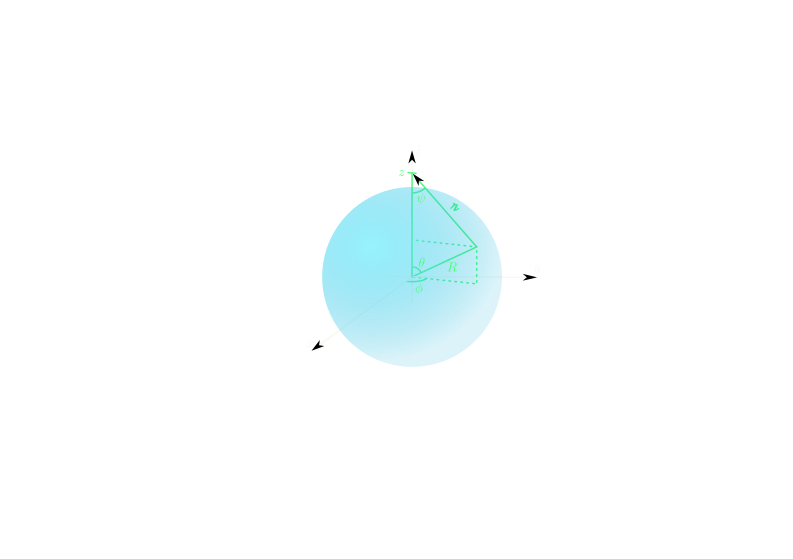
\includegraphics[width=0.5\linewidth]{images/fig2_7.png}
    \captionsetup{width=0.8\linewidth}
    \caption{An electric field a distance $z$ from the center of a spherical surface of radius $R$
    that carries a charge density $\sigma$.}
    \label{fig:2_7}
\end{figure}
Once again, the electric field is in the $z$-direction:
\begin{equation}
    \vb{E} = \frac{1}{4\pi\epsilon_0}   
    \int \frac{\sigma}{\scriptr^2} \cos\psi \vu{z} \dd{\vb{a}}
\end{equation}
From the law of cosines, $\scriptr^2 = z^2 + R^2 - 2zR\cos\theta$; Geometrically,
$\cos\psi = \dfrac{z - R \cos\theta}{\scriptr}$; the surface area element is
$\dd{\vb{a}} = R^2 \sin\theta \dd{\theta} \dd{\theta}$:
\begin{align*}
    \vb{E} &=  \ke\int_0^{2\pi} \int_0^{\pi}
        \frac{\sigma R^2(z - R \cos\theta)}{(z^2 + R^2 - 2zR\cos\theta)^{3/2}}
        \sin\theta \dd{\theta} \dd{\phi} \vu{z} \\
        &= \ke (2\pi\sigma R^2) \int_0^{\pi}
        \frac{z - R \cos\theta}{(z^2 + R^2 - 2zR\cos\theta)^{3/2}}
        \sin\theta \dd{\theta} \vu{z} \\
        &= \ke (2\pi\sigma R^2) f(\theta) \vu{z}
\end{align*}
using the substitution $u = \cos\theta$: $\dd{u} = -\sin\theta \dd{\theta}$, and the limits of
integration are $[\cos{0}, \cos{\pi}]$. So,
\begin{align*}
    f(\theta) =
    \int_{-1}^{1} \frac{z - Ru}{(z^2 + R^2 - 2zRu)^{3/2}} \dd{u} = f(u)
\end{align*}
substituting again with $v = \sqrt{z^2 + R^2 - 2zRu}$; $\dd{v} = -\dfrac{zR}{v} \dd{u}$; and $
u = \dfrac{1}{2zR}(z^2 + R^2 - v^2)$:
\begin{align*}
    f(v) &= -\frac{1}{zR} \int \frac{z - \frac{1}{2z}(z^2 + R^2 - v^2)}{v^3} v \dd{v} \\
    &= -\frac{1}{2z^2R} \int \frac{2z^2 - (z^2 + R^2 - v^2)}{v^2} \dd{v} \\
    &= -\frac{1}{2z^2R} \int \frac{v^2 + z^2 - R^2}{v^2} \dd{v} \\
    &= -\frac{1}{2z^2R} \int \qt(1 + \frac{z^2 - R^2}{v^2}) \dd{v} \\
    &= -\frac{1}{2z^2R} \qt(v - \frac{z^2 - R^2}{v})
\end{align*}
back substituting $v = \sqrt{z^2 + R^2 - 2zRu}$,
\begin{align*}
    f(u) &= -\frac{1}{2z^2R} \qt(\frac{z^2 + R^2 - 2zRu}{\sqrt{z^2+R^2-2zRu}} 
        - \frac{z^2 - R^2}{\sqrt{z^2 + R^2 - 2zRu}}) \eval_{-1}^1 \\
    &= -\frac{1}{2z^2R} \qt(\frac{2R^2 - 2zRu}{\sqrt{z^2+R^2-2zRu}}) \eval_{-1}^1 \\
    &= \frac{1}{z^2} \qt(\frac{zu - R}{\sqrt{z^2+R^2-2zRu}}) \eval_{-1}^1 \\
    &= \frac{1}{z^2} \qt(
        \frac{z - R}{\sqrt{z^2 + R^2 - 2zR}} - \frac{-z - R}{\sqrt{z^2 + R^2 + 2zR}}
    )
\end{align*}
Taking the positive square root: $\sqrt{z^2 + R^2 - 2zR} = (R - z)$ if $R > z$, but $(z - R)$ if
$R < z$. So, for the case $z < R$ (inside the sphere) the electric field is
\begin{align*}
    \vb{E} &= \frac{1}{4\pi\epsilon_0} \frac{2\pi\sigma R^2}{z^2} \qt(
        \frac{z - R}{R - z} - \frac{-z - R}{R + z}
    ) \vu{z} \\
    &= \frac{1}{4\pi\epsilon_0} \frac{2\pi\sigma R^2}{z^2} \qt(
        \frac{z - R}{R - z} + \frac{z + R}{R + z}
    ) \vu{z} \\
    &= \frac{1}{4\pi\epsilon_0} \frac{2\pi\sigma R^2}{z^2} \qt(
        \frac{z - R}{R - z} + 1
    ) \vu{z} \\
    &= \frac{1}{4\pi\epsilon_0} \frac{2\pi\sigma R^2}{z^2} \qt(
        \frac{z - R}{R - z} + \frac{R - z}{R - z}
    ) \vu{z} \\
    &= 0
\end{align*}
For the case $z > R$ (outside the sphere) the electric field is
\begin{align*}
    \vb{E} &= \ke \frac{2\pi\sigma R^2}{z^2} \qt(
        \frac{z - R}{z - R} + \frac{z + R}{z + R}
    ) \vu{z} \\
    &= \ke \frac{4\pi\sigma R^2}{z^2} \vu{z} \\
    &= \ke \frac{q}{z^2} \vu{z}
\end{align*}
This makes sense: From outside the sphere, the point charge $q$ is the
charge-per-area $\sigma$ times the surface area of the sphere $4\pi R^2$, or simply
$q = 4\pi R^2 \sigma$.

\paragraph{2.8}
Finding the field inside and outside a solid sphere of radius $R$ with a uniform volume charge
density $\rho$ is similar to Prob. 2.7. Outside the solid sphere the total charge $q$ contributes
to the electric field as if it were a point charge:
\begin{align*}
    \vb{E}_{out} &= \ke \frac{q}{r^2} \vu{r}
\end{align*}
Inside the solid sphere, only the volume of the solid sphere less than $r$ contributes to the
electric field. The volume of the total sphere is $V = \frac{4}{3}\pi R^3$, and the volume of the
sphere less than $r$ is $V' = \frac{4}{3}\pi r^3$. So, electric field inside the solid sphere is
\begin{align*}
    \vb{E}_{in} &= \frac{V'}{V} \vb{E}_{out} \\
    &= \frac{r^3}{R^3} \ke \frac{q}{r^2} \vu{r} \\
    &= \ke \frac{q}{R^3} r \vu{r}
\end{align*}
or
\begin{align*}
    \vb{E}_{in} = \ke \frac{q}{R^3} \vb{r}
\end{align*}

\paragraph{2.9}
(a) The electric field in some region is $\vb{E} = kr^3 \vu{r}$ in spherical coordinates, where
$k$ is a constant. The differential form of Gauss's law is
\begin{align*}
    \div{\vb{E}} &= \frac{\rho}{\epsilon_0}
\end{align*}
and the radial component of divergence in spherical coordinates is
\begin{align*}
    [\div{\vb{E}}]_r &= \frac{1}{r^2} \pdv{r} (r^2 E_r) \\
    &= \frac{1}{r^2} \pdv{r} (r^2 kr^3) \\
    &= 5kr^2
\end{align*}
So, the charge density is
\begin{align*}
    \rho &= 5\epsilon_0 kr^2
\end{align*}
(b) The total charge inside a sphere of radius $R$ is found using Gauss's law:
\begin{align*}
\oint \vb{E} \vdot \dd{\vb{a}} &= \frac{Q}{\epsilon_o} \\
Q &= \epsilon_o \oint \vb{E} \vdot \dd{\vb{a}} \\
&= \epsilon_o \int (kR^3 \vu{r}) \vdot (R^2 \sin\theta \dd{\theta} \dd{\phi} \vu{r}) \\
&= \epsilon_o \int_0^{2\pi} \int_0^\pi (kR^5 \sin\theta) \dd{\theta} \dd{\phi} \\
&= 4\pi \epsilon_o k R^5
\end{align*}
or using Gauss's theorem:
\begin{align*}
    \oint \vb{E} \vdot \dd{\vb{a}} &= \int (\div \vb{E}) \dd{\tau} \\
    Q &= \epsilon_o \int_0^{2\pi} \int_0^\pi \int_0^R
        5kr^2 (r^2 \sin\theta) \dd{r} \dd{\theta} \dd{\phi} \\
    &= 4\pi \epsilon_o k R^5
\end{align*}

\paragraph{2.10}
For simplicity, using a cube of length 1:
\begin{align*}
    y = 1 ,\quad \vb{E} = \ke \frac{q(x\vu{x} + y\vu{y} + z\vu{z})}{r^3}
    ,\quad \dd{a} = \dd{x} \dd{z} \vu{y} ;\quad \vb{E} \vdot \dd{a} = \ke \frac{q}{r^3}
\end{align*}
the limits of integration are $x = [0,1]$ and $z = [0,1]$:
\begin{align*}
    \oint \vb{E} \vdot \dd{a} &=\ke q \int \frac{1}{r^3} \dd{x} \dd{z} \\
    &= \ke q \int_0^1 \int_0^1 \frac{1}{(x^2 + 1 + z^2)^{3/2}} \dd{x} \dd{z} \\
    &= \ke q \int_0^1 \qt[
        \frac{x}{(1+z^2) \sqrt{x^2 + 1 + z^2}} \eval_0^1 
    ] \dd{z} \\
    &= \ke q \int_0^1 \frac{1}{(1 + z^2) \sqrt{2 + z^2}} \dd{z} \\
    &= \ke q \arctan(\frac{z}{\sqrt{z^2 + 2}}) \eval_0^1 \\
    &= \ke q \qt(\frac{\pi}{6}) = \frac{q}{24\epsilon_o}
\end{align*}
Where the first integral is solved using the trig identity $x = \tan(u) \sqrt{z^2 + 1}$, and 
similarly, the second integral uses $z = \tan(u) \sqrt{2}$.

\begin{figure}[ht]
    \centering
    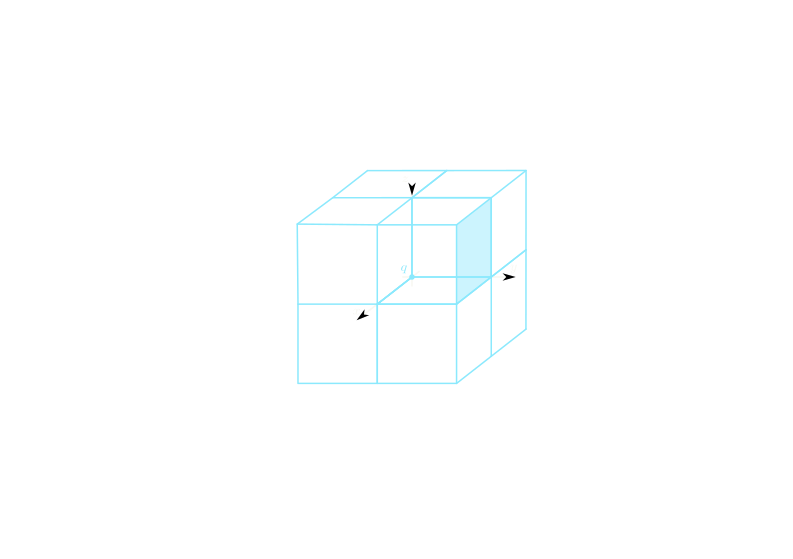
\includegraphics[width=0.5\linewidth]{images/fig2_10.png}
    \captionsetup{width=0.8\linewidth}
    \caption{8 cubes with a charge $q$ at the center.}
    \label{fig:2_10}
\end{figure}
The simpler solution is though the superposition of 8 cubes with the charge in the center of the
larger cube, and the surface that encloses the larger cube is made of 24 squares equivalent to the
shaded region as shown in Figure \ref{fig:2_10}. Therefore, the flux through the shaded region is
$\frac{1}{24}$ of the total flux $\frac{q}{\epsilon_o}$.

\paragraph{2.11}
For a spherical shell of radius $R$ with a uniform surface charge density $\sigma$, the enclosed
charge in side the sphere is $Q_{enc} = 0$, thus the electric field inside the sphere is 
\begin{align*}
    \vb{E}_i = 0
\end{align*}
and using the sphericla symmetry of a Gaussian surface, the electric field outside the sphere is
\begin{align*}
    \oint \vb{E}_o \vdot \dd{\vb{a}} &= \frac{1}{\epsilon_o} Q_{enc} \\
    \abs{\vb{E}_0} \int \dd{\vb{a}} &= \frac{1}{\epsilon_o} (4\pi\sigma R^2) \\
    \vb{E}_o (4\pi r^2) &= \frac{1}{\epsilon_o} (4\pi\sigma R^2) \vu{r} \\
    \vb{E}_o &= \frac{\sigma R^2}{\epsilon_o r^2} \vu{r}
\end{align*}

\paragraph{2.12}
Inside a solid sphere, the total charge enclosed in the Gaussian surface is
\begin{align*}
    Q_{enc} &=  V'\rho = \frac{4}{3} \pi r^3 \rho
\end{align*}
where $V'$ is the volume of the sphere enclosed by the Gaussian surface. Using Gauss's law,
\begin{align*}
    \oint \vb{E} \vdot \dd{\vb{a}} = \frac{1}{\epsilon_o} Q_{enc}
    = \frac{1}{\epsilon_o} \frac{4}{3} \pi r^3 \rho
\end{align*}
using the spherical symmetry of the Gaussian surface, the electric field is
\begin{align*}
    \oint \vb{E} \vdot \dd{\vb{a}} = \abs{\vb{E}} \int \dd{a} 
    = \abs{\vb{E}} (4\pi r^2)
\end{align*}
Thus
\begin{align*}
    \abs{\vb{E}} (4\pi r^2) = \frac{1}{\epsilon_o} \frac{4}{3} \pi r^3 \rho
\end{align*}
or
\begin{align*}
    \vb{E} = \frac{1}{3\epsilon_o} r \rho \vu{r} = \frac{1}{3\epsilon_o} \rho \vb{r}
\end{align*}
Since the total charge of the solid sphere is $q = \frac{4}{3} \pi R^3 \rho$, the electric field
can be rewritten as
\begin{align*}
    \vb{E} = \ke \frac{q}{R^3} \vb{r}
\end{align*}
which is the same as Prob. 2.8.

\paragraph{2.13}
Finding the electric field a distance $s$ from an infinitely long straight wire that carries a
uniform line charge $\lambda$. Using a Gaussian cylinder of radius $s$ and length $L$, 
enclosed charge is $Q_{enc} = \lambda L$. Using Gauss's law and the symmetry of the cylinder,
\begin{align*}
    \oint \vb{E} \vdot \dd{\vb{a}} &= \frac{1}{\epsilon_o} Q_{enc} \\
    \abs{\vb{E}} \int \dd{s'}\dd{\phi'}\dd{z'} &= \frac{1}{\epsilon_o} \lambda L \\
    E (2\pi s L) &= \frac{1}{\epsilon_o} \lambda L
\end{align*}
or
\begin{align*}
    \vb{E} = \frac{\lambda}{2\pi\epsilon_o s} \vu{s} = \ke \frac{2\lambda}{s} \vu{s}
\end{align*}
which is similar to Eq. 2.9.

\paragraph{2.14}
Find the electric field inside a sphere that carries a charge density proportional to the distance
from the origin, $\rho = kr$, where $k$ is a constant: The enclosed charge is
\begin{align*}
    Q_{enc} = \int \rho \dd{\tau} = \int_0^{2\pi} \int_0^\pi \int_0^r kr (r^2 \sin\theta) \dd{r}
        \dd{\theta} \dd{\phi} = \pi k r^4
\end{align*}
Using Gauss's law and the spherical symmetry of the Gaussian surface,
\begin{align*}
    \oint \vb{E} \vdot \dd{\vb{a}} &= \frac{1}{\epsilon_o} Q_{enc} \\
    \abs{\vb{E}} \int \dd{a} &= \frac{1}{\epsilon_o} \pi k r^4 \\
    E (4\pi r^2) &= \frac{1}{\epsilon_o} \pi k r^4
\end{align*}
or 
\begin{align*}
    \vb{E} = \frac{1}{4\pi\epsilon_o} \pi k r^2 \vu{r} = \ke kr\vb{r}
\end{align*}

\paragraph{2.15}
A thick spherical shell with charge density
\begin{align*}
    \rho = \frac{k}{r^2} \quad (a\leq r \leq b)
\end{align*}
The electric field in the three regions: \\
(i) \(r<a\)
\[ Q_{enc} = 0; \vb{E} = 0 \]

(ii) \(a\leq r \leq b\)
\[ Q_{enc} = \int_0^{2\pi} \int_0^\pi \int_a^r \rho (r^2 \sin\theta) \dd{r} \dd{\theta} \dd{\phi}
= 4\pi \int_a^r \frac{k}{r^2} (r^2) \dd{r} = 4\pi k (r - a) \]
And from Gauss's law,
\begin{align*}
    \oint \vb{E} \vdot \dd{\vb{a}} &= \frac{1}{\epsilon_o} Q_{enc} \\
    \abs{\vb{E}} \int \dd{a} &= \frac{1}{\epsilon_o} 4\pi k (r - a) \\
    E (4\pi r^2) &= \frac{1}{\epsilon_o} 4\pi k (r - a)
\end{align*}
or 
\begin{align*}
    \vb{E} &= \frac{k (r - a)}{\epsilon_o r^2} \vu{r} = \ke \frac{4\pi k(r - a)}{r^3} \vb{r}
\end{align*}

(iii) \(r>b\)
\[ Q_{enc} = \int_0^{2\pi} \int_0^\pi \int_a^b \rho (r^2 \sin\theta) \dd{r} \dd{\theta} \dd{\phi}
= 4\pi k (b - a) \]
And from Gauss's law,
\begin{align*}
    \oint \vb{E} \vdot \dd{\vb{a}} &= \frac{1}{\epsilon_o} Q_{enc} \\
    \abs{\vb{E}} \int \dd{a} &= \frac{1}{\epsilon_o} 4\pi k (b - a) \\
    E (4\pi r^2) &= \frac{1}{\epsilon_o} 4\pi k (b - a)
\end{align*}
or
\begin{align*}
    \vb{E} &= \frac{k (b - a)}{\epsilon_o r^2} \vu{r} = \ke \frac{4\pi k(b - a)}{r^3} \vb{r}
\end{align*}
\begin{figure}[ht]
    \centering
    \includegraphics[width=0.5\linewidth]{images/fig2_15.png}
    \captionsetup{width=0.8\linewidth}
    \caption{Plot of $\abs{\vb{E}}$ as a function of $r$, for the case $b = 2a$.}
    \label{fig:2_15}
\end{figure}

\paragraph{2.16}
A long coaxial cable carries a uniform \emph{volume} charge charge density $\rho$ on the inner
cylinder (radius $a$), and a uniform \emph{surface} charge density $\sigma$ on the outer cylindrical
shell (radius $b$). This surface charge is negative, and the cable as a whole is electrically
neutral. Find the electric field in the three regions:

(i) Inside the inner cylinder \(r < a\): The enclosed charge is
\begin{align*}
    Q_{enc} = \rho \pi s^2 l
\end{align*}
where l is the length of the Gaussian cylinder. Using Gauss's law,
\begin{align*}
    \oint \vb{E} \vdot \dd{\vb{a}} &= \frac{1}{\epsilon_o} Q_{enc} \\
    \abs{\vb{E}} \int \dd{a} &= \frac{1}{\epsilon_o} \rho \pi s^2l \\
    E (2\pi sl) &= \frac{1}{\epsilon_o} \rho \pi s^2l \\
    \vb{E} = \frac{\rho s}{2\epsilon_o} \vu{s}
\end{align*}

(ii) Between the cylinders \(a \leq r \leq b\): The enclosed charge is
\[ Q_{enc} = \rho \pi a^2 l \]
thus the electric field is
\begin{align*}
    E (2\pi sl) &= \frac{1}{\epsilon_o} \rho \pi a^2 l \\
    \vb{E} = \frac{\rho a^2}{2\epsilon_o s} \vu{s}
\end{align*}

(iii) Outside the cable \(r > b\): The enclosed charge is
\[ Q_{enc} = \rho \pi a^2 l - \sigma \pi b l  = 0\]
thus the electric field is
\( \vb{E} = 0 \)

\begin{figure}[ht]
    \centering
    \includegraphics[width=0.5\linewidth]{images/fig2_16.png}
    \captionsetup{width=0.8\linewidth}
    \caption{Plot of $\abs{\vb{E}}$ as a function of $r$, for the case $b = 2a$.}
    \label{fig:2_16}
\end{figure}

\paragraph{2.17}
Finding the electric field, as a function of $y$, where $y=0$ is the center of an infinite plane
slab, of thickness $2d$, carrying a uniform volume charge density $\rho$. For the case \(y > 2d\)
The enclosed charge is
\begin{align*}
    Q_{enc} = \rho (2d) A = 2\rho Ad
\end{align*}
where $A$ is the area of the Gaussian pillbox. Using Gauss's law,
\begin{align*}
    \oint \vb{E} \vdot \dd{\vb{a}} &= \frac{1}{\epsilon_o} Q_{enc} \\
    \abs{\vb{E}} \int \dd{a} &= \frac{1}{\epsilon_o} 2\rho Ad \\
    E (2A) &= \frac{1}{\epsilon_o} 2\rho Ad \\
    \vb{E} &= \frac{\rho d}{\epsilon_o} \vu{y}
\end{align*}
For the case \(0 < y < 2d\), the enclosed charge is
\begin{align*}
    Q_{enc} = 2\rho y A
\end{align*}
and the electric field is
\begin{align*}
    E (2A) &= \frac{1}{\epsilon_o} \rho y A \\
    \vb{E} &= \frac{\rho y}{\epsilon_o} \vu{y}
\end{align*}
In the $-y$ direction, $E$ is negative as shown in Figure \ref{fig:2_17}.
\begin{figure}
    \centering
    \includegraphics[width=0.5\linewidth]{images/fig2_17.png}
    \captionsetup{width=0.8\linewidth}
    \caption{Plot of $\abs{\vb{E}}$ as a function of $y$}
    \label{fig:2_17}
\end{figure}

\paragraph{2.18}
For two spheres of radius $R$ and charge density $+\rho$ and $-\rho$, respectively, are partially
overlapping. From Prob 2.12, the electric field inside a sphere of radius $R$ with a uniform volume
charge density $\rho$ is
\[ \vb{E} = \frac{1}{3\epsilon_o} \rho \vb{r} \]
where $\vb{r}$ is the position vector from the center of the sphere. The electric field for each 
sphere is
\begin{align*}
    \vb{E}_1 &= \frac{1}{3\epsilon_o} \rho \vb{r}_1 \\
    \vb{E}_2 &= -\frac{1}{3\epsilon_o} \rho \vb{r}_2
\end{align*}
Thus the total electric field is
\begin{align*}
    \vb{E} &= \frac{1}{3\epsilon_o} \rho (\vb{r}_1 - \vb{r}_2) \\
    &= \frac{1}{3\epsilon_o} \rho \vb{d}
\end{align*}
where $\vb{d}$ is the vector from the positive center to the negative center. Thus the electric
field is constant inside the overlapping region.

\paragraph{2.19}
The electric field inside a sphere of radius $R$ with a uniform volume charge density $\rho$ is
\[\tag{2.8} \label{eq:2_8}
\vb{E}(r) = \ke \int \frac{\hat \boldscriptr}{\scriptr^2} \rho(\vb{r}') \dd{\tau'}
\]
The curl of \eqref{eq:2_8} is
\[
\curl \vb{E} = \ke \int \curl \qt(\frac{\hat \boldscriptr}{\scriptr^2}) \rho(\vb{r}') \dd{\tau'}
\]
From Prob 1.63, \( \curl \frac{\hat \boldscriptr}{\scriptr^2} = 0 \), thus
\[ \curl \vb{E} = 0 \]
\end{document}